\documentclass[aspectratio=169]{beamer}
% Bullet, label and outline shapes: each frame checks that the shape, colour and size of
% list bullets and outline markers survive in Slides, next to the item text.
\usetheme{Madrid}
\usepackage{amssymb}
\usepackage{pifont}
\title{Bullet shapes}
\author{Test}
\date{}

\begin{document}

\section{Itemize}
\subsection{Templates}

{
\setbeamertemplate{itemize items}[triangle]
\begin{frame}{Triangles}
  \begin{itemize}
    \item First level
      \begin{itemize}
        \item Second level
          \begin{itemize}
            \item Third level
          \end{itemize}
      \end{itemize}
    \item Back to the first
  \end{itemize}
\end{frame}
}

{
\setbeamertemplate{itemize items}[circle]
\setbeamercolor{item}{fg=red}
\begin{frame}{Red circles}
  \begin{itemize}
    \item First level
      \begin{itemize}
        \item Second level
          \begin{itemize}
            \item Third level
          \end{itemize}
      \end{itemize}
    \item Back to the first
  \end{itemize}
\end{frame}
}

{
\setbeamertemplate{itemize items}[square]
\setbeamercolor{item}{fg=green!50!black}
\begin{frame}{Green squares}
  \begin{itemize}
    \item First level
      \begin{itemize}
        \item Second level
          \begin{itemize}
            \item Third level
          \end{itemize}
      \end{itemize}
    \item Back to the first
  \end{itemize}
\end{frame}
}

{
\setbeamertemplate{itemize items}[ball]
\setbeamercolor{item projected}{bg=orange}
\begin{frame}{Orange balls}
  \begin{itemize}
    \item First level
      \begin{itemize}
        \item Second level
          \begin{itemize}
            \item Third level
          \end{itemize}
      \end{itemize}
    \item Back to the first
  \end{itemize}
\end{frame}
}

\subsection{Custom}

{
\setbeamertemplate{itemize item}{\textcolor{orange}{$\blacktriangleright$}}
\setbeamertemplate{itemize subitem}{\textcolor{blue}{$\star$}}
\setbeamertemplate{itemize subsubitem}{\ding{51}}
\begin{frame}{Custom glyphs}
  \begin{itemize}
    \item An orange triangle
      \begin{itemize}
        \item A blue star
          \begin{itemize}
            \item A dingbat check mark
          \end{itemize}
      \end{itemize}
    \item[\ding{43}] A pointing hand
    \item[$\diamond$] A diamond
    \item[\textcolor{purple}{$\blacksquare$}] A purple square
    \item[{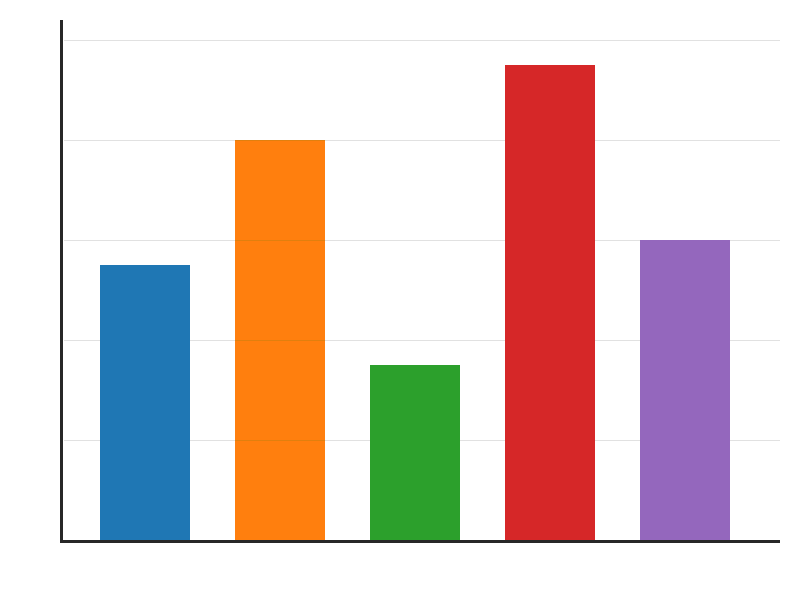
\includegraphics[height=1.6ex]{img/plot.png}}] A picture as a bullet
  \end{itemize}
\end{frame}
}

\section{Enumerate}

{
\setbeamertemplate{enumerate items}[circle]
\renewcommand\theenumi{\roman{enumi}}
\begin{frame}{Roman numbers on circles}
  \begin{enumerate}
    \item First
    \item Second
    \item Third
    \item Fourth
  \end{enumerate}
\end{frame}
}

{
\setbeamertemplate{enumerate items}[square]
\renewcommand\theenumi{\alph{enumi}}
\begin{frame}{Letters on squares}
  \begin{enumerate}
    \item First
    \item Second
      \begin{enumerate}
        \item Nested
      \end{enumerate}
    \item Third
  \end{enumerate}
\end{frame}
}

{
\setbeamertemplate{enumerate items}[ball]
\begin{frame}{Three digits and large items}
  \begin{enumerate}
    \setcounter{enumi}{98}
    \item Ninety-nine
    \item One hundred
    \item One hundred and one
  \end{enumerate}
  \begin{columns}[T]
    \column{0.45\textwidth}
    \large
    \begin{enumerate}
      \item Large one
      \item Large two
    \end{enumerate}
    \column{0.45\textwidth}
    \begin{enumerate}
      \item Right one
      \item Right two
    \end{enumerate}
  \end{columns}
\end{frame}
}

\section{Description}

{
\setbeamercolor{description item}{fg=teal}
\begin{frame}{Description lists}
  \begin{description}
    \item[Shape] The form of the marker
    \item[Colour] Its fill, taken from the page
    \item[] An item without a label
    \item<2->[Later] Shown from the second step
  \end{description}
  \begin{itemize}
    \item[] An itemize item with an empty label
    \item<2-> An item uncovered later
  \end{itemize}
\end{frame}
}

\section{Outline}
\subsection{Balls}
\subsection{Circles}

{
\setbeamertemplate{sections/subsections in toc}[ball]
\begin{frame}{Outline with balls}
  \tableofcontents
\end{frame}
}

{
\setbeamertemplate{sections/subsections in toc}[circle]
\begin{frame}{Outline with circles}
  \tableofcontents
\end{frame}
}

{
\setbeamertemplate{sections/subsections in toc}[square]
\setbeamercolor{subsection in toc}{fg=red!70!black}
\begin{frame}{Outline with squares}
  \tableofcontents[currentsection]
\end{frame}
}

\begin{frame}{Outline in two columns}
  \begin{columns}[T]
    \column{0.45\textwidth}
    \tableofcontents[sections={1-2}]
    \column{0.45\textwidth}
    \tableofcontents[sections={3-4}]
  \end{columns}
\end{frame}

\end{document}
